\section{Metodologia}


\begin{frame}

    \frametitle{Metodologia}

    Para a escolha dos algoritmos foi utilizado o Princípio da Descrição de Comprimento Mínimo (DCM) da mesma forma que foi utilizado na tese de Proença \cite{proencca2021robust}.
    \newline
    \newline
    Para guiar o processo de criação da arquitetura foi utilizado a metodologia \textit{Goal Question Metric (GQM)} \cite{caldiera1994goal}, metodologia muito utilizada no campo da Engenharia de Software \cite{sommerville2011software}.

\end{frame}

\subsection{Arquitetura de Dutos e Filtros}
\begin{frame}

    \frametitle{Estrutura da Arquitetura de Dutos e Filtros}

    \begin{figure}[!htbp]
                \centering
       	    \caption{Exemplo de um pipeline}
       	    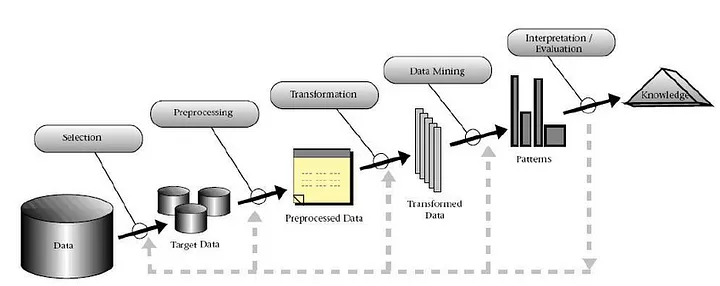
\includegraphics[scale=0.65]{imagens/pipeline.png}
            \end{figure}

\end{frame}


\begin{frame}
    \frametitle{Definição das Fases}
     \begin{itemize}
        \item Pré-Processamento
            \begin{itemize}
                \item Uso da ferramenta \textbf{GritBot} da RuleQuest Research para detectar anomalias (\textit{outliers}).
            \end{itemize}
            
        \item Transformação
            \begin{itemize}
                \item \textbf{\textit{Outlier}}: Maiores áreas construídas;
                \item \textbf{Item}: Tipo Construtivo X Padrão de Acabamento X \textit{Outlier};
                \item \textbf{Transações}: agrupamento por CEP;
                \item \textbf{Utilidade}: área construída;
                \item \textbf{Utilidade Negativa}: área do terreno vago;
            \end{itemize}
    \end{itemize}
\end{frame}

\begin{frame}
    \frametitle{Mineração de Dados}
     \begin{itemize}
        \item Algoritmos
            \begin{itemize}
                \item \textbf{FPClose} - Algoritmo eficiente para obter os itemsets fechados mais frequêntes;
                \item \textbf{OpusMiner} - Algorigmo para obter os itemsets estatisticamente relevantes;
                \item \textbf{FHM Freq} - Algoritmo para obter os itemsets de maior utilidade e suporte.
                \item \textbf{FHN} - Algoritmo para processar itemsets de utilidade negativa;
                \item \textbf{Cortana} - \textit{Software} para processar subgrupos de interesse.
            \end{itemize}
    \end{itemize}
\end{frame}